\chapter{A Técnica de Reconstrução}
	\label{capituloReconstrucao}

Em posse do referencial teórico descrito no capítulo \ref{capituloReferencialTeorico}, a reconstrução de um objeto se deu através da indicação de pontos de interesse na imagem e da implementação de hipóteses de restrição geométrica, baseadas na transformação de câmera encontrada, a fim de eliminar a multiplicidade inerente às correspondência projetiva (seção \ref{secaoProjecoes}).

	Inicialmente, é necessário descobrir qual matriz de transformação projetiva é capaz de gerar tal imagem do objeto. Tal conhecimento permite conhecer a posição 2D, no sistema de coordenadas e sob mesmo ponto de vista da imagem, que corresponde a qualquer ponto 3D do espaço. Como discutido na seção \ref{secaoCalibracao}, 6 correspondências entre pontos 2D e 3D, conhecidas previamente, são o bastante para fornecer uma aproximação da transformação desejada; no entanto, neste trabalho são usadas 8 correspondências, obrigatoriamente entre os pontos 3D:
	\begin{itemize}
		\item (0,0,0);
		\item (1,0,0);
		\item (0,1,0);
		\item (1,1,0);
		\item (0,0,1);
		\item (1,0,1);
		\item (0,1,1);
		\item (1,1,1).
	\end{itemize}
	Tal restrição tem o intuito de simplificar a entrada de dados do usuário no aplicativo de reconstrução (seção \ref{appReconstrucao}) e garantir a satisfação da condição de independência linear para a boa execução do método de calibração (seção \ref{secaoCalibracao}).
	
	Após o processo de calibração já é possível descobrir se um ponto 3D tem sua projeção coincidente com um ponto de interesse na imagem, podendo, por força-bruta, inferir a posição 3D no espaço deste ponto de interesse, 2D, da imagem. 
	
	No entanto, resta, ainda, o problema da multiplicidade de pontos; sabendo-se que isto se dá devido a formação da imagem ser feita através da interseção entre a reta de projeção (reta que liga o ponto 3D retratado ao centro de projeção da câmera) e o plano de projeção (figura \ref{imagemProjecaoConica}).
	
	Analisando o cenário que contém o objeto, nota-se que a reta de projeção contém vários pontos 3D, mas cada um destes tem um valor exclusivo da coordenada $Z$ (figura \ref{imagemUnicoPontoPorPlano}); isto é provado pela geometria analítica, uma vez que a interseção entre uma reta (a reta de projeção, no caso) e um plano (no caso, um plano $Z = k$, com um $k$ qualquer) é um ponto.
	
	\begin{figure}[!htb]
		\centering
		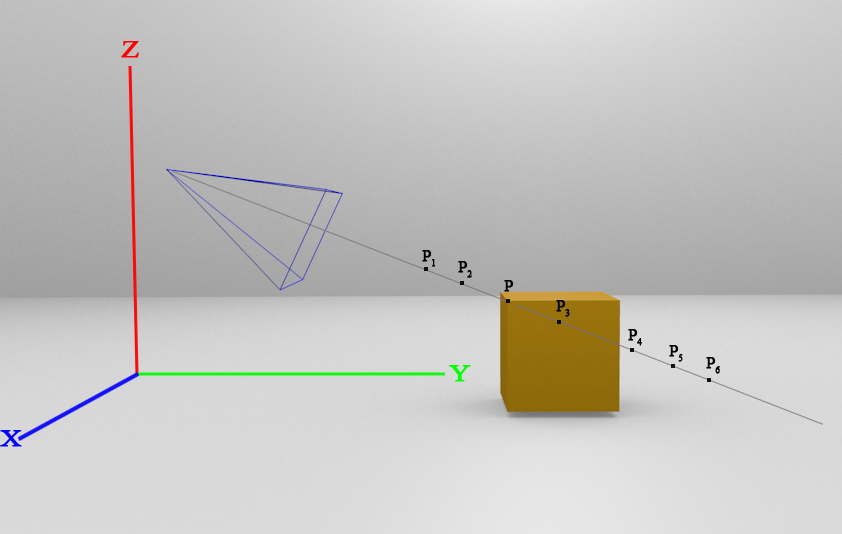
\includegraphics[height=5.5cm]{imagens/cenaExemploUnicoPontoPorPlano.png}
		\caption{Os pontos $P_i$ pertencem à reta de projeção de $P$, mas suas coordenadas Z são diferentes da coordenada Z do ponto $P$}
		\label{imagemUnicoPontoPorPlano}
	\end{figure}
	
	Se, ao indicar o ponto de interesse, fosse fornecido o seu valor da coordenada Z, determinar seu correspondente 3D no espaço seria uma tarefa banal com uma demanda exaustiva por dados do usuário. Em viés, sem informações além da transformação projetiva e coordenadas 2D do ponto de interesse não há formas de determinar sua coordenada Z \cite{foto3D}.
	
	No entanto, devido ao apelo visual da imagem, é fácil determinar se um ponto da imagem tem seu correspondente 3D com coordenada Z igual, ou aceitavelmente igual, à coordenada Z do correspondente 3D de outros pontos da imagem (figura \ref{imagemPontosMesmoPlano}). De forma que, ao fornecer os pontos de interesse para a reconstrução, indicar quais pontos de interesse da imagem têm seu correspondente 3D em uma mesma coordenada Z é simples e provê subterfúgios para a eliminação da multiplicidade projetiva.
	
	Neste trabalho, para cada grupamento é atribuído um identificador numérico inteiro, onde, quanto menor o identificador, menor a coordenada Z do grupamento.
	
	\begin{figure}[!htb]
		\centering
		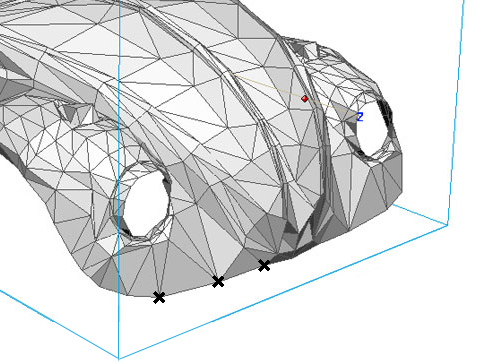
\includegraphics[height=5cm]{imagens/pontosMesmoPlano.png}
		\caption{É perceptível que os pontos demarcados com um "X" têm a mesma coordenada Z no espaço}
		\label{imagemPontosMesmoPlano}
	\end{figure}
	
	Assim, de posse de um grupamento de pontos da imagem com mesma coordenada Z, iterativamente, são descartados valores para a coordenada Z do grupamento que cujo plano no espaço, pela transformação projetiva encontrada para a imagem, não possui um ponto possível de ser o correspondente 3D de algum dos pontos de interesse do grupamento em questão.
	
	Tal eliminação de multiplicidade por interseção é eficaz dado o seu embasamento geométrico citado anteriormente. No entanto, assim como no estabelecimento das correspondências (seção \ref{secaoCalibracao}), há imprecisão na demarcação dos pontos de interesse na imagem. Então, é compreensível que seja adotada uma tolerância projetiva. A tolerância projetiva diz respeito a quão longe do ponto demarcado como interessante à reconstrução um ponto 3D ainda pode projetar para ser considerado como correspondente a este; tolerâncias grandes levam à imprecisão de reconstrução, ao passo que tolerâncias pequenas levam à dificuldade em achar correspondentes. O valor da tolerância projetiva é definido pelo usuário no momento da reconstrução. 
	
	Tal tolerância pode causar a não convergência da eliminação por interseção para um único valor; neste caso, o valor da coordenada Z adotado é dado por um critério de convergência arbitrário como valor mais próximo ao plano anteriormente analisado ou valor mais próximo da média entre os possíveis valores encontrados.
	
	Ainda em consequência da tolerância projetiva, com a coordenada Z adotada um número finito de pontos com esta coordenada Z projetam próximo o suficiente do ponto de interesse. Assim, como correspondente 3D definitivo do ponto de interesse em questão é adotado o baricentro destes pontos.
	
	Não obstante, é necessário que se determine um espaço finito de busca destes correspondentes 3D, já que há pontos 3D que projetam em um ponto de interesse em infinitas posições do espaço. Para limitar a busca, então, são usados os mesmo pontos 3D aplicados na correspondência para calibração, isto é, os pontos $P = {(x, y, z) | 0 \leq x, y, z \leq 1}$. Como resultado, os pontos 3D reconstruídos terão suas coordenadas entre 0 e 1.
	
	Dentro do espaço de busca, um quesito ainda importante é a distância ente dois valores consecutivos de uma coordenada (i.e. incremento). Incrementos menores levam à uma maior precisão da reconstrução, enquanto incrementos maiores tornam o algoritmo mais ágil. O valor do incremento é definido no início da recosntrução.
	
	Em suma, é importante ressaltar que esta técnica reconstrói apenas pontos 3D, arestas e planos podem ser adicionados à nuvem de pontos resultado em um processo de pós-tratamento.
	
	